% ----------------------------------------------------------------------
% Section 3 — Technical Concept
% ----------------------------------------------------------------------
\section{Technical Concept}\label{sec:technical_concept}
% TODO: remove section information
High-level, technology-agnostic view of the system. This section
introduces the conceptual building blocks and the end-to-end data
flow. Detailed component-level descriptions follow in the Hardware,
AWS Services, and User Interaction sections.

\subsection{Technical Building Blocks}\label{sec:building_blocks}
% TODO: remove section information
Enumerate the logical components of the system without binding them
yet to concrete products: edge sensing node, secure transport channel,
ingestion gateway, validation stage, hot-path store (live data),
cold-path store (history), query API, notification channel, and user
interface. Briefly justify the chosen programming languages
(C++ firmware, Python lambdas, TypeScript infrastructure, React UI).

\subsection{System Architecture}\label{sec:architecture}
\begin{figure*}[!tb]
  \centering
  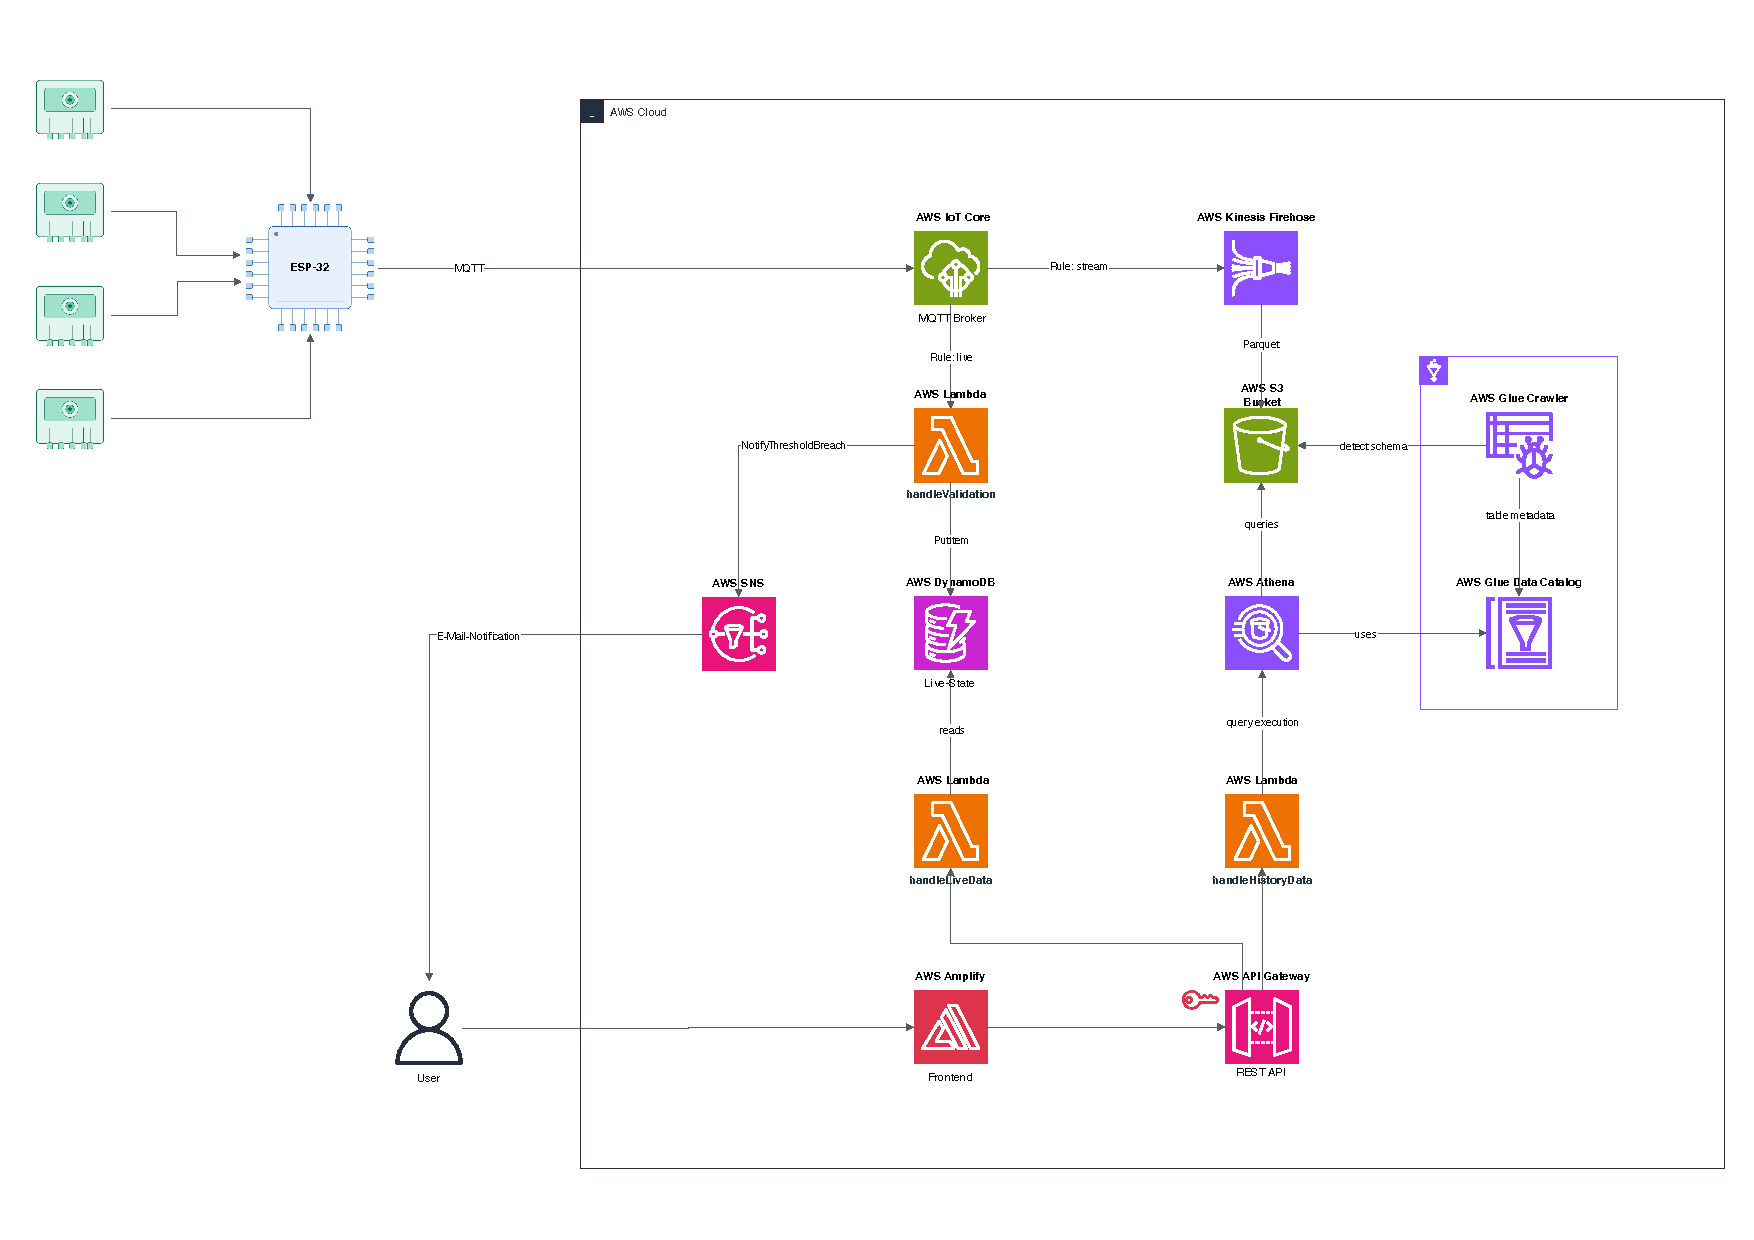
\includegraphics[width=\textwidth]{architecture.pdf}
  \caption{Cloud Processing Architecture}
  \label{fig:cloud-architecture}
\end{figure*}
